\chapter{Appendix}
\label{sec:appendix}

% Slightly larger size for the table
\begin{table}[H]
\caption{Questions of questionnaire}
\resizebox{\textwidth}{!}{%
\begin{minipage}{\textwidth}
\footnotesize  % Slightly larger font size than \small
\begin{longtable}{|p{5cm}|p{9cm}|}  % Increased column width to 6cm
\hline
\textbf{Question} & \textbf{Answer} \\
\hline
\endfirsthead

\hline
\textbf{Question} & \textbf{Answer} \\
\hline
\endhead

\hline
\endfoot

\hline
Wie alt sind Sie? & Number \\
\hline
Was ist Ihr Geschlecht? & Männlich / Weiblich / Divers / Keine Angabe \\
\hline
Für was für eine Art von Studium sind Sie derzeit eingeschrieben? & Bachelor / Master / Ich studiere nicht \\
\hline
In welcher Universität sind Sie eingeschrieben? & Text \\
\hline
In welchem Studiengang sind Sie eingeschrieben? & Text \\
\hline
In welchem Semester befinden Sie sich? & Number \\
\hline
Wie viel Erfahrung haben Sie mit Programmieren? & Keine Erfahrung / Weniger als 1 Jahr / 1-2 Jahre / 3-5 Jahre / Mehr als 5 Jahre \\
\hline
Ihre Einschätzung Ihrer Fähigkeiten in Java. & Keine Kenntnisse / Grundkenntnisse / Durchschnittliche Kenntnisse / Gute Kenntnisse / Sehr gute Kenntnisse \\
\hline

"Beschreiben Sie in wenigen Worten oder Sätzen, was der Code Ihrer Meinung nach tut." & Text \\
\hline
"Wie sicher fühlen Sie sich bei Ihrer Antwort zur ersten Frage?" & Sehr unsicher / Unsicher / Neutral / Sicher / Sehr sicher \\
\hline
"Wie verständlich ist der Code für Sie?" & Sehr unverständlich / Unverständlich / Neutral / Verständlich / Sehr verständlich \\
\hline
"Wie beurteilen Sie die Kommentierung des Codes?" & Verwirrend, überflüssig oder unverständlich / Nicht optimal, könnte ausführlicher sein / Neutral / Angemessen, erleichtert das Verständnis / Hilfreich und klar \\
\hline
"Wie beurteilen Sie die Einrückung des Codes?" & Unlesbar / Schlecht lesbar / Neutral / Gut lesbar / Sehr gut lesbar \\
\hline

Was zeichnet für Sie gut kommentierten Code aus? & Text \\
\hline
Was zeichnet für Sie schlecht kommentierten Code aus? & Text \\
\hline
Inwieweit achten Sie darauf, Kommentare gemäß den zuvor von Ihnen definierten Richtlinien zu schreiben? & Nie / Selten / Manchmal / Oft / Immer \\
\hline
Wenn Sie Code schreiben, wie gestalten Sie die Einrückung? & Ich achte nicht bewusst auf die Einrückung. / Ich verwende die Tab-Taste. / Ich rücke manuell mit Leerzeichen ein. / Ich nutze die automatische Formatierung meiner IDE. / Ich passe die Einrückung an den Stil des Projekts an. / Ich kombiniere Tabs und Leerzeichen. / Ich kopiere Einrückungen aus vorhandenen Codebeispielen. / Ich verwende ein spezielles Code-Formatierungs-Tool (z. B. Prettier, Black, Clang-Format) \\
\hline
E-Mail-Adresse für MMI-Punkte erhalten / Gutschein-Verlosung & Text \\
\hline
\end{longtable}
\end{minipage}%
} 
\end{table}

\begin{figure}[H]
    \centering
    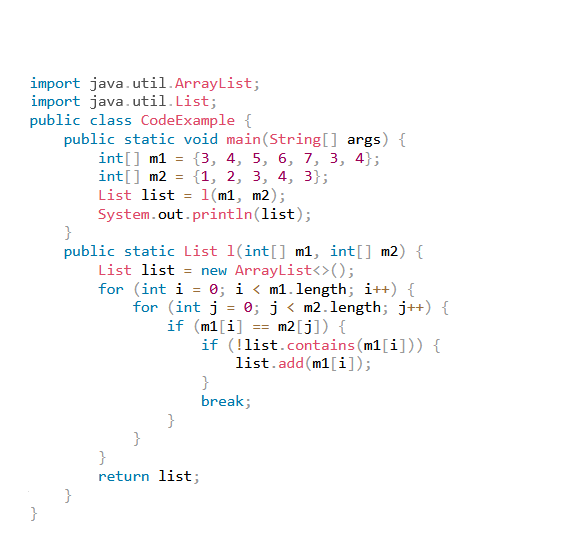
\includegraphics[width=0.6\textwidth]{figures/schnitt.png}
    \caption{Code snippet 1}
    \label{fig:appendix-example1}
\end{figure}

\begin{figure}[H]
    \centering
    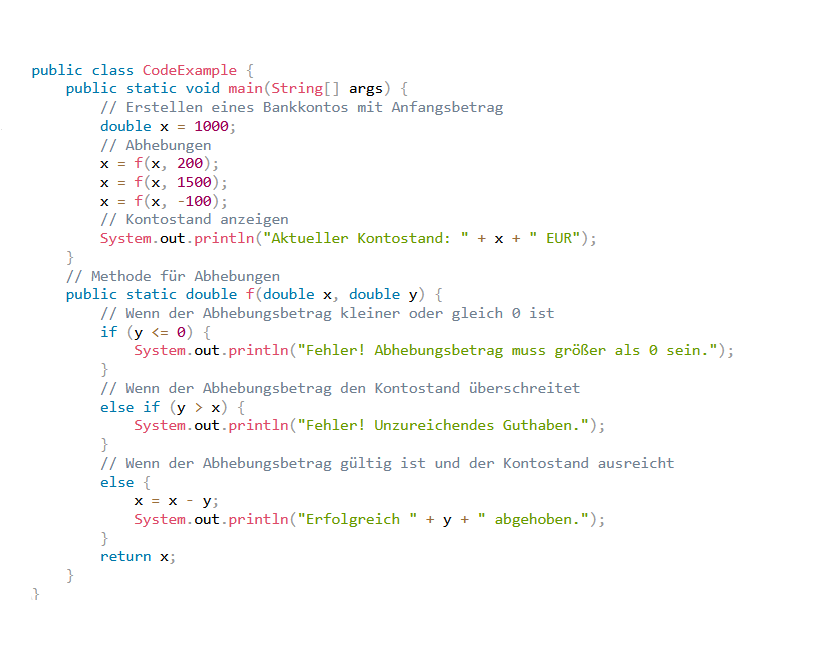
\includegraphics[width=0.9\textwidth]{figures/konto.png}
    \caption{Code snippet 2}
    \label{fig:appendix-example2}
\end{figure}

\begin{figure}[H]
    \centering
    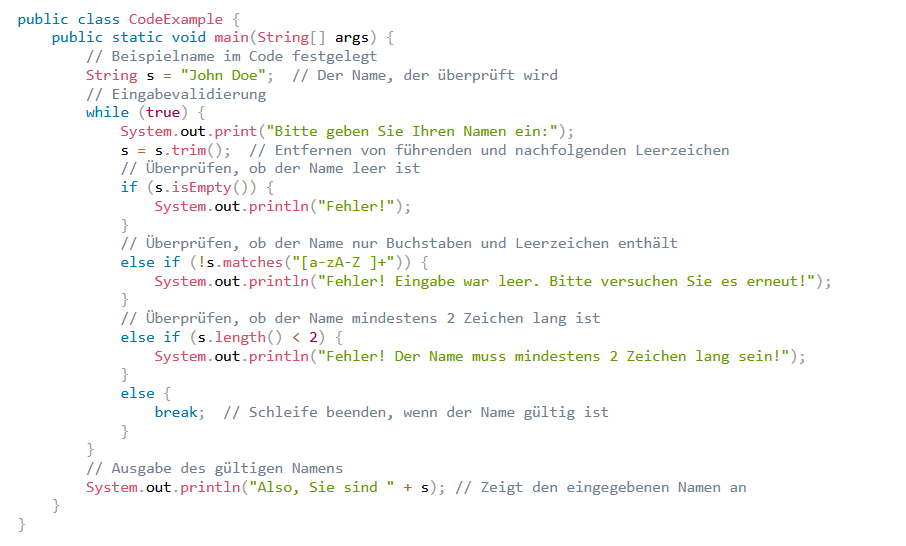
\includegraphics[width=0.9\textwidth]{figures/name.png}
    \caption{Code snippet 3}
    \label{fig:appendix-example3}
\end{figure}


\begin{figure}[H]
    \centering
    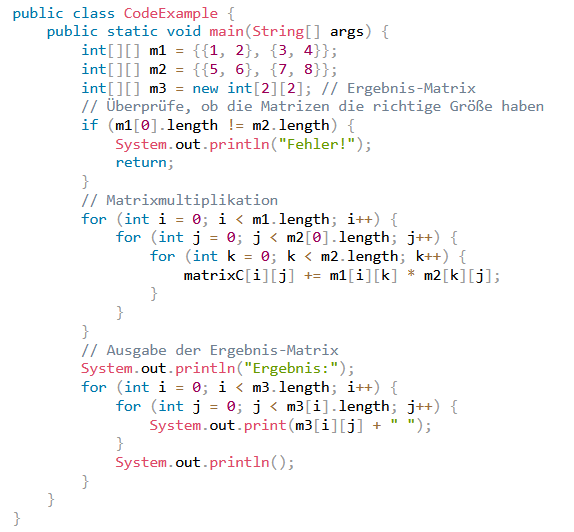
\includegraphics[width=0.7\textwidth]{figures/m.png}
    \caption{Code snippet 4}
    \label{fig:appendix-example4}
\end{figure}

\begin{figure}[H]
    \centering
    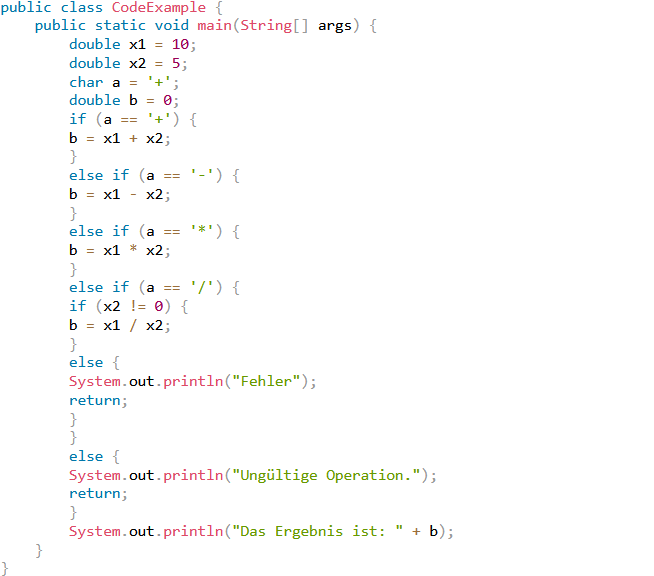
\includegraphics[width=0.8\textwidth]{figures/rechner.png}
    \caption{Code snippet 5}
    \label{fig:appendix-example5}
\end{figure}


\begin{figure}[H]
    \centering
    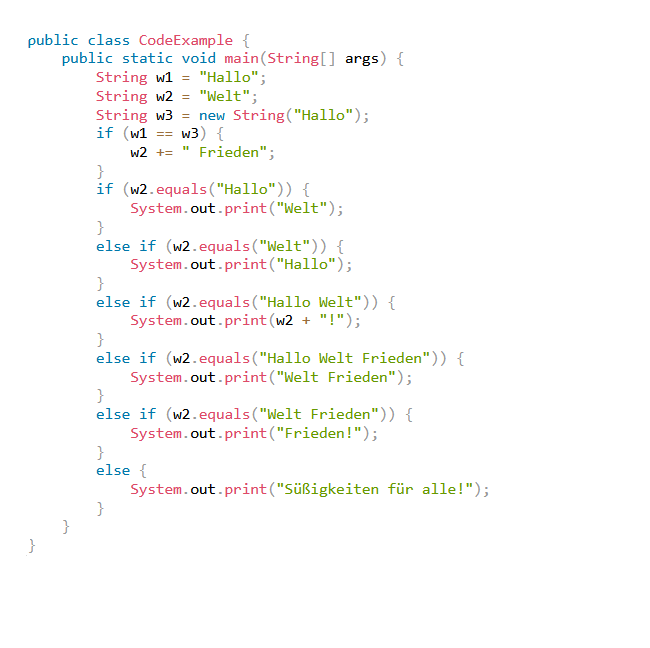
\includegraphics[width=0.8\textwidth]{figures/hello.png}
    \caption{Code snippet 6}
    \label{fig:appendix-example6}
\end{figure}


\begin{figure}[H]
    \centering
    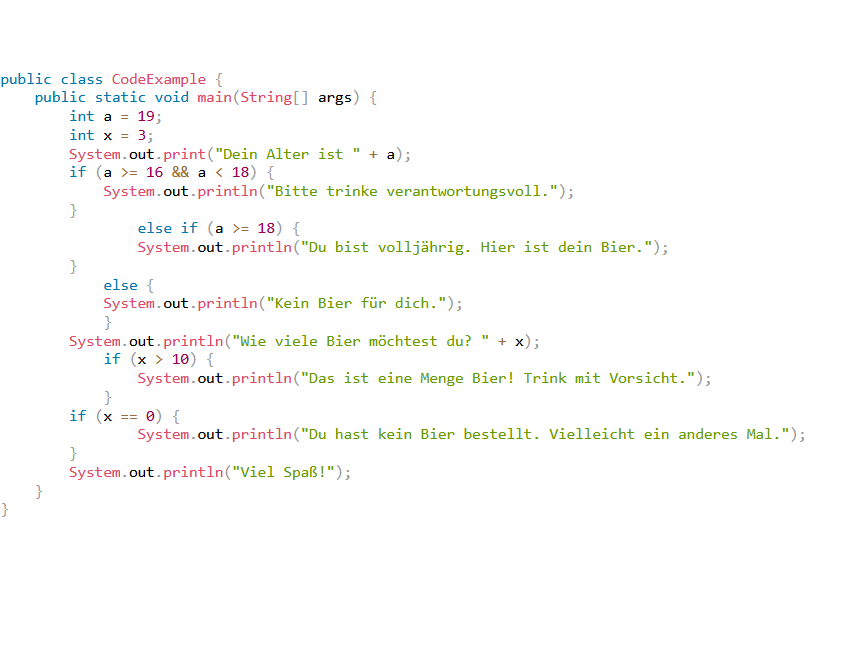
\includegraphics[width=0.9\textwidth]{figures/bier.png}
    \caption{Code snippet 7}
    \label{fig:appendix-example7}
\end{figure}

\thispagestyle{plain}